\documentclass[11pt]{article}
	\usepackage{xcolor}
    \title{\textbf{User Story Example}}
    \author{Justal Kevin}
    \date{22 January 2020}
    
    \addtolength{\topmargin}{-3cm}
    \addtolength{\textheight}{3cm}
\usepackage{graphicx}
\begin{document}

\maketitle
\thispagestyle{empty}

\section{Preface}
The goal of this document is to give everyone an idea of what could be an user story well detailed for a very smooth implementation for the frontend and backend. At the end of the document, the reader should have no question because all of them are already answered in the document. For this example, I will take something that everybody know : the chat of messenger.\\

\section{Prerequisit}
I consider the app installed by the users on their phone and already have an account setup. An account alias user has \textbf{an username} and a \textbf{password}.

\section{Limitation}
I will limit the function to \textbf{a chat} when a \textbf{logged user} can read and write a \textbf{message}. There is no search on the previous \textbf{message}. No edit or delete of the \textbf{message}. I will also not talk about the login functionnalities. It's part of another functionnalities who will describe how to login, not here.

\section{Goal}
The goal is to allow a \textbf{logged user} to send a \textbf{message} to another \textbf{logged user}.

\section{Personna}

There is only two kind of user possible in this function :

\begin{itemize}
  \item \textbf{Logged user}
  \item \textbf{Not logged user}
\end{itemize}

\section{Permissions}

\subsection{Permission of an user on his \textbf{message}}

\begin{table}[!htb]
	\centering
	\begin{tabular}{|c|c|c|c|}
		\hline
		& Read & Write \\  [0.5ex]
		\hline 
		Logged user & Yes & Yes \\ 
		\hline 
		Not logged user & No & No \\ 
		\hline 
	\end{tabular} 
    \label{table:nonlin}
\end{table}

\subsection{Permission of an user on the \textbf{message} of someone else}

\begin{table}[!hbt]
	\centering
	\begin{tabular}{|c|c|c|}
		\hline
		& Read & Write \\  [0.5ex]
		\hline 
		Logged user & Y & No \\ 
		\hline 
		Not logged user & No & No \\ 
		\hline 
	\end{tabular} 
	\label{table:nonlin}
\end{table}

\section{Flowchart}

\begin{figure}[htp]
\centering
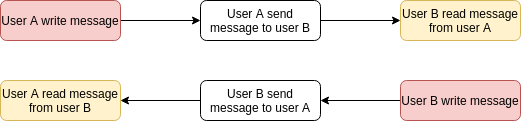
\includegraphics[scale=0.50]{images/whatever.png}
\caption{}
\label{}
\end{figure}

\section{Stories}

For those stories, we will follow those users :

\begin{table}[!hbt]
	\centering
	\begin{tabular}{|c|c|}
		\hline
		username & password \\  [0.5ex]
		\hline 
		 Robert & azerty \\  
		\hline 
		 Nicolas & drtyu \\  
		\hline 
	\end{tabular} 
	\label{table:nonlin}
\end{table}

\subsection{Robert want to send a \textbf{message} to Nicolas - both logged and present}

Robert and Nicolas are logged in the app and chatting together.

\begin{itemize}
  \item \emph{Robert logged to his account by using his username and password}.
  \item Once logged, Robert write a \textbf{message} by typing on the keyboard and press the button send for sending the \textbf{message}
  \item The \textbf{message} of Robert is shown to the app of Nicolas.
\end{itemize}

\subsection{Robert want to send a \textbf{message} to Nicolas - Nicolas not logged}

Robert is logged in the app but Nicolas is not logged.

\begin{itemize}
  \item \emph{Robert logged to his account by using his username and password}.
  \item Once logged, Robert write a \textbf{message} by typing on the keyboard and press the button send for sending the \textbf{message}
  \item The \textbf{message} of Robert is waiting for Nicolas to logged before he can see it. \color{blue}A notification can be shown on the phone of Nicolas.
\end{itemize}

\subsection{Robert want to send without logged or has no account}

Robert want to send without logged or has no account

\begin{itemize}
  \item \emph{Robert cannot access the app for sending a \textbf{message}}.
\end{itemize}

\subsection{Robert want to send a \textbf{message} to Nicolas but lost internet}

Robert send a \textbf{message} but lost internet just before sending a \textbf{message}

\begin{itemize}
  \item \emph{Robert logged to his account by using his username and password}.
  \item Once logged, Robert write a \textbf{message} by typing on the keyboard and press the button send for sending the \textbf{message}
  \item The \textbf{message} is waiting on the app of Robert for \color{red}30 seconds max.\color{black}
  \item Once Robert get internet back, the \textbf{message} is sent to Nicolas.
  \item If robert does not have internet before the end of the 30s, the \textbf{message} is deleted and will not be send.
\end{itemize}

\section{Code}

\begin{itemize}
  \item \textbf{Bold text} : A bold text indicate more details are given into the definition section.
  \item \textbf{Italic text} : An italic text indicate a functionnality describe in another document.
  \item \textbf{Blue text} : A blue text indicate a functionnality not needed by the client but could be a good thing to have.
  \item \textbf{Red text} : A red text indicate a parameter the client can change.
\end{itemize}

\section{Definitions}
\begin{itemize}
  \item \textbf{Logged user} : An user who has connect logged to the app with his username and password.
  \item \textbf{Not logged user} : An user who has connect to the app and try to do some action.
  \item \textbf{username} : The name that will be use in the application and the name use for login
  \item \textbf{password} : The password use by the user for login to the app
  \item \textbf{message} : A paragraph with a date for ordering the message by latest
  \item \textbf{chat} : Exchange of message
\end{itemize}

\section{Question}

This part should stay empty after the project has started. If modifications or questions are added here, it means the document was poorly made in the first place. No questions should result after reading the document because all question are already answered in the document.

\end{document}

